\newpage
\section{Постановка задачі}

\subsection{Проблема навігації робота}

У цій роботі ми розглянемо проблему навігації агента (робота) в умовах середовища, заповненого перешкодами. Ми спробуємо створити адаптивну систему контролю агента (робота), завданням якого є самостійних рух у віртуальному середовищі, оминання перешкод, що зустрічаються на його шляху та якомога швидше добирання до заданого пункту призначення. Щоб якомога краще наблизити поведiнку автопiлота до людської поведiнки, система керування роботом сприймає лише об’єкти, якi потрапляють у поле зору, обмежене певним кутом та дальнiстю огляду. Базуючись на цій обмеженій інформації, навчена система контролю повинна бути здатна ефективно керувати роботом і приводити його без зіткнень з перешкодами до заданої мети.

За останні роки цю задачу пробували розв'язувати багатьма різними способами. Більшість цієї роботи було сконцентровано на плануванні шляху, коли повністю відоме середовище аналізується для того, щоб знайти оптимальний шлях до мети. Це, наприклад, метод обчислення потенціальних полів, які ``відштовхують'' робота від перешкоди і ``притягують'' до цілі або метод дискретизації  простору для того, щоб здійсювати швидкий пошук вільних від перешкод траекторій. Обмеженням цих методів в тому, що вони потребують попередніх повних знань про розташування перешкод в середовищі, і, відповідно, кожен раз, як змінюється їх конфігурації, потребують повного переобчисленння. Також, знайдені оптимальні траекторії абсолютно не враховують динаміки самого робота, тому необхідним стає розроблення ще одного контролера, який би відповідав за проведення робота запланованою траекторією.

На противагу цим методам, реактивні контролери використовують лише поточний стан системи, який вони здатні сприймати, для того, щоб зробити рішення про наступну дію. В результаті здійснення кожної дії відбувається зміна стану, і, відповідно, здійснюється рішення про дію в новій ситуації. Для прикладу, системи на основі бази знань опираються на заздалегідь визначені правила поведінки для того, щоб зробити рішення про наступну дію. В такому підході розробник повинен в своїх правилах враховувати динаміку робота і, відповідно, підлаштовувати їх для кожного конкретного застосування.

Поставлена задача "--- одна з тих, в яких можна з успіхом застосувати методику навчання з підсиленням. Перевагою цього підходу є те, що система самотійно вчиться досягати мети, використовуючи будь-яку інформацію про стан системи та наявні дії. В умовах обмеженої та неповної інформації розробляється поведінка, яка максимально враховує та використовує усю надану інформацію. Більш детальний огляд методів розв'язування даної задачі можна знайти у \cite{Rummery1995}.

\subsection{Дедуктивні та індуктивні методи навчання}

Серед широкого спектру методів та підходів, розроблених в рамках машинного навчання, можна виділити дві групи методів, які кардинально відрізняються у своєму підході до проблеми набуття агентом знань. Це "--- індуктивні та дедуктивні методи навчання.

З цих двох груп методів найбільш дослідженими та теоретично обґрунтованими є дедуктивні методи навчання, основна ідея яких полягає в тому, що для того, щоб навчити агента діяти ``інтелектуально'' в умовах зовнішнього середовища, потрібно заздалегідь надати йому певну експертну інформацію, тобто інформацію, зібрану, опрацьовану та структуровану людьми, які є спеціалістами в даній галузі. Такі методи навчання ще називають навчанням із вчителем (supervised learning), оскільки необхідною умовою успіху є наявність певного ``вищого інтелекту'', який володіє знаннями і передає їх агенту. Для дедуктивних методів надзвичайно важливим є питання повноти експертних знань, їх коректності та точності. При цьому основним питанням, поряд з проблемою ефективних методів навчання на основі зібраної інформації, виступає проблема підготовки та організації готових знань, її структуризація таким чином, щоб вона могла бути якомога ефективніше використана агентом під час попереднього навчання.

На відміну від дедуктивних методів, індуктивні методи намагаються уникнути необхідності у попередніх знаннях. При цьому, якщо попередні знання присутні, вони можуть бути певним чином ``інтегровані'' в агента, тим самим додаткову інформацію також можливо ефективно використати. Але при цьому, навіть при відсутності готових знань, правил, індуктивні методи дають можливість агенту самому виробити ефективну та ``розумну'' поведінку шляхом багаторазової взаємодії з зовнішнім середовищем. В результаті численних спроб та помилок, агент здатний на основі набутого ``досвіду'' виробити власну стратегію оптимальної поведінки. Тобто агент, завдяки індуктивному навчанню, вибудовує внутрішню модель поведінки, базуючись лише на отриманому в результаті взаємодії з середовищем досвіді.

\subsection{Порівняння з попереднім підходом}

Ми вже намагалися розв'язати схожу задачу дедуктивним методом навчання, а саме використовуючи нейромережу та навчальну вибірку як експертну систему для розроблення системи контролю автомобіля. Щоправда, поставлена задача дещо відрізнялася в тому, що від автомобіля вимагалося лише оминання перешкоди, без чітко зазначеного кінцевого пункту призначення. Задача ускладнювалася більш реалістичною фізикою руху автомобіля, аніж у задачі контролю роботом, що розглядається у цій роботі. Оскільки керування роботом не вимагає великих швидкостей, ми припускаємо, що здатні повертати робот на заданий кут, залишаючись при цьому на місці, а також здатні миттєво зупинятися або ж, навпаки, рушати. У випадку з автомобілем ці припущення були б дещо нереалістичними, тому у фізиці автомобіля присутні інерція та швидкість руху, а також реалістичне здійснення повороту.

Отримані результати в задачі контролю автомобілем важко охарактеризувати однозначно. З однiєї сторони, система контролю на базi нейромережi досить адекватно керувала автомобiлем з доволі складною фізикою, успiшно оминаючи перешкоди та забезпечуючи безперервний рух автомобiля в середовищi, про яке вона не мала жодної попередньої iнформацiї. Базуючись лише на даних про вiддаль до найближчих об’єктiв в полi зору, система контролю забезпечувала завчасне оминання перешкоди з плавною змiною швидкостi та напрямку руху автомобiля. Очевидно, що велику роль в досягненнi вказаної природностi та адекватностi керування вiдiграла вдало пiдiбрана навчальна множина.

З iншого боку, найбiльшою проблемою, з якою довелося зiткнутися, була наявнiсть ситуацiй, в яких автомобiль зупинявся i система контролю не могла вивести його з нерухомого стану. Це, зокрема, ситуацiя, подана на рис.~\ref{car_stuck}, в якiй автомобiль заїхав у глухий кут i застряг, не зумiвши здiйснити розворот назад. Цю проблему, теоретично, можна було б розв'язати, ввівши у визначення стану автомобіля значення поточної швидкості та задавши додаткові набори ключових експертних правил, які б дозволили автомобілю здійснити розворот у разі застрягання в глухому куті. Проте на практиці це достатньо проблематично, оскільки введення додаткової змінної стану призводить до ускладення поведінки всієї системи, підвищення рівня вимог до точності та репрезентативності експертних правил. Також для того, щоб зробити розворот автомобіля безпечнішим та природнішим, довелося б вводити також змінні, які б відповідали за задній огляд автомобіля, що призводить до ще більш строгих вимог до експертних правил.

\begin{figure}
	\centering
    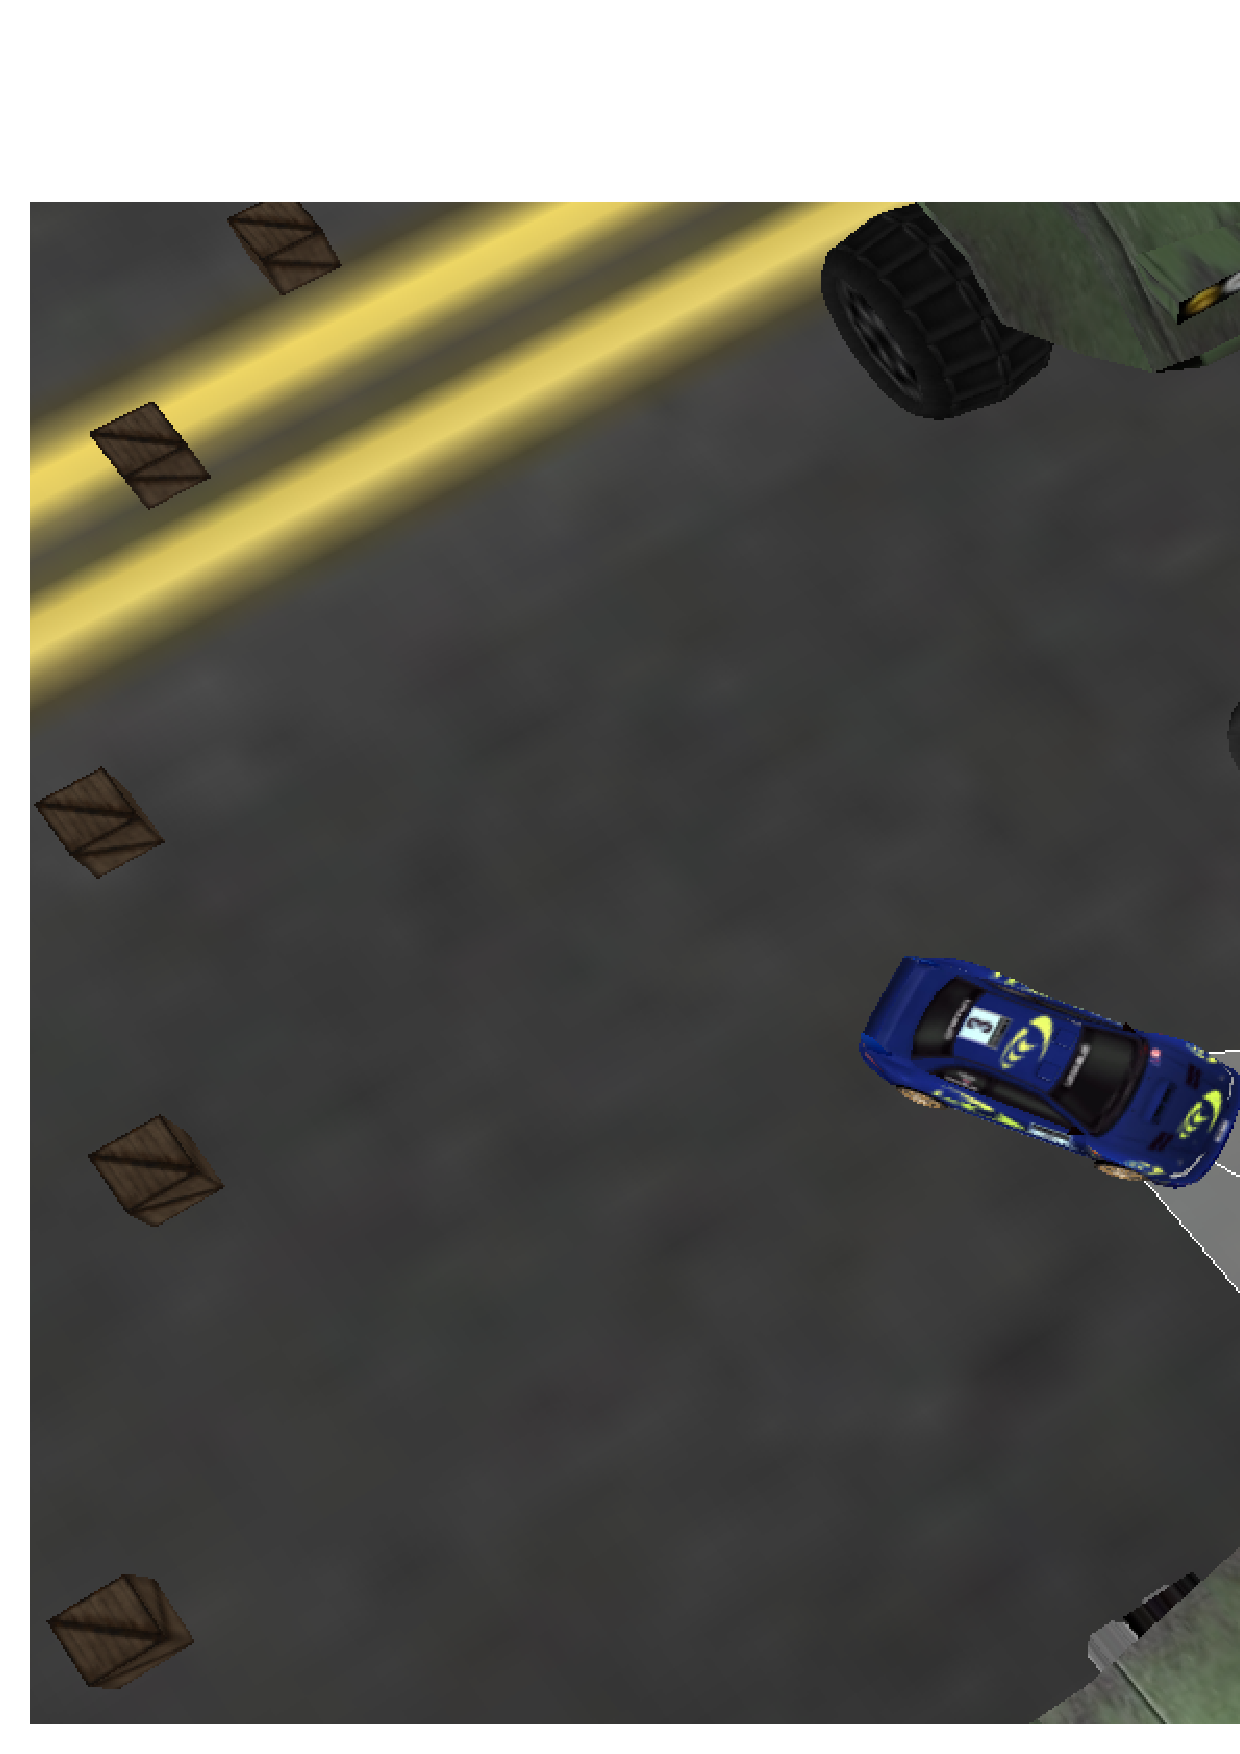
\includegraphics[width=0.6\textwidth]{stuck.png}
	\caption{Автомобіль застряг, заїхавши у кут}
	\label{car_stuck}
\end{figure}


Слiд зазначити, що ще однiєю причиною (окрiм вказаної обмеженостi визначеного стану динамiчної системи) такої поведiнки є особливiсть фiзичної моделi автомобiля. Мається на увазi природа автомобiля "--- для того щоб здiйснити поворот, чи, тим бiльше, розворот, автомобiль повинен здiйснювати поступальний рух, що в умовах, коли вже вiдбулося ``застрягання'', дуже проблематично. Можливим розв’язанням даної проблеми є змiна типу транспортного засобу. Якщо взяти транспортний засiб, здатний здiйснювати поворот без поступального руху (як у випадку з роботом), то можна значно зменшити ймовiрнiсть його застрягання. Таким транспортним засобом, для прикладу, може бути танк, в якому шляхом незалежного обертання гусениць в рiзнi сторони можна домогтися розвороту на будь-який кут, залишаючись при цьому на мiсцi.

Важливою проблемою є вибір внутрішньої структури нейромережі. Якщо використати недостатню кількість нейронів та внутрішніх прошарків, то нейромережа не зможе в достатній мірі вивчити набір правил і, таким чином, не зможе повністю використати експертні знання. З іншого боку, використовуючи надто велику кількість нейронів, існує загроза надто точного запам'ятовування (overfitting) правил без належного узагальнення їх на схожі ситуації. В такому випадку нейромережа буде добре поводитися у ситуаціях, заданих в експертних правилах, але навіть незначна зміна ситуації приведе до абсолютно неадекватної поведінки, яка значно відрізняється від заданої для близької еталонної ситуації.

Таким чином, при використанні наперед заданих експертних правил, з'являється велика кількість практичних питань, на які немає чітких теоретичних відповідей, а все доводиться вирішувати в результаті численних експериментів. Саме тому було вирішено відійти від підходу, який базується на заздалегідь відібраних експертних знаннях, а піти шляхом самоорганізації "--- дати можливість агенту розробити власну систему правил на основі отриманого внаслідок взаємодії з середовищем досвіду.

\subsection{Індуктивний підхід "--- навчання з підсиленням}

Оскільки використання попереднього підходу сильно залежить від якості навчальної вибірки (експертних правил), що при найменшому ускладненні сприйняття агентом середовища призводить до значних ускладнень експертних правил, було вирішено відійти від моделі навчання з учителем. Натомість був використаний самоорганізаційний підхід. Основна ідея такого підходу полягає в тому, щоб дати можливість агенту розробити власну систему правил щодо оптимальної поведінки в умовах середовища, завдяки безпосередній взаємодії з середовищем. Взаємодіючи з середовищем, агент отримує певний досвід і, якщо задати певний механізм оцінки агентом власних дій, то в результаті достатньої кількості ``досвіду'', можна надіятися, що агент розробить ефективну стратегію поведінки. Такий підхід отримав назву \emph{навчання з підсиленням (reinforcement learning)}. При використанні навчання з підсиленням відпадає необхідність в складному і трудомісткому процесі розробки системи якісних і репрезентативних експертних правил, хоча, натомість, з'являєть необхідність в виборі механізму оцінки дій агента. Проте, для достатньо складних систем зазвичай значно легше визначити механізм безпосередньої оцінки дій, аніж розробити достатньо повну та якісну систему правил.

Розглянемо застосування такого індуктивного процесу навчання (на відміну від дедуктивного на базі системи правил) до вищезазначеної задачі навігації агента.

\subsection{Середовище}

\begin{figure}
	\centering
    \includegraphics[width=0.7\textwidth]{env_screen.png}
	\caption{Віртуальне середовище}
	\label{fig:environment}
\end{figure}

Для випробування вищезазначеної ідеї було створено віртуальне середовище (див. рис.~\ref{fig:environment}). Робот має п'ять секторів огляду, в межах яких він сприймає точну відстань до найближчої перешкоди. Центральний кут кожного сектору складає 18\textdegree. Таким чином робот сприймає об'єкти в межах поля зору в 90\textdegree. Роботу надається інформація про кут між напрямком його руху та напрямком на ціль, а також відстань до цілі (рис.~\ref{fig:perception}). Таким чином, робот сприймає середовище як багатовимірний неперервний простір.

\begin{figure}
	\centering
    \includegraphics[width=0.7\textwidth]{perception.png}
	\caption{Сприймання роботом середовища}
	\label{fig:perception}
\end{figure}

Середовище становить собою квадратну кімнату, в якій знаходять випадково згенеровані та розташовані перешкоди, що являють собою опуклі многокутники. Уся дія відбувається епізодами. Робот починає на початку кожного епізоду свій рух у випадковій позиції з випадковим початковим напрямом руху і повинен дістатися вказаної точки, яка також генерується випадково, не натикаючись на межі кімнати та на перешкоди.

Робот рухається, вибираючи на кожному кроці дію з дискретної множини допустимих дій, а саме:
\begin{itemize}
	\item рухатись прямо на невелику відстань;
	\item рухатись прямо на невелику відстань, одночасно повернувши наліво на невеликий кут повороту;
	\item рухатись прямо на невелику відстань, одночасно повернувши направо на невеликий кут повороту;
	\item залишитися на місці, повернувши наліво на невеликий кут повороту;
	\item залишитися на місці, повернувши направо на невеликий кут повороту.
\end{itemize}

Робот робить рішення про наступний хід доти, доки не буде виконана одна з наступних умов:
\begin{itemize}
	\item досягнуто цілі;
    \item зіткнення з перешкодою або межею кімнати;
	\item перевищено ліміт кількості кроків;
\end{itemize}

В усіх цих випадках епізод вважається закінченим. Після цього знову генерується випадковий епізод і все повторюється з початку.

\subsection{Деталі реалізації}

В нашій програмній реалізації було використано алгоритм Sarsa для навчання. Параметр дисконтування $\gamma$ було прийнято рівним $0.99$ для того, щоб враховувати якомога краще можливі наслідки прийнятих дій.

За кожен крок агент отримував винагороду, рівну $-0.01$, таким чином ми намагалися домогтися такої послідовності дій, яка б вела до цілі за найменшу кількість кроків. При досягненні мети, отримувалася нагорода, рівна $1.00$. При зіткненні з перешкодою, покарання було найбільшим і становило:
\[
    -1+ \frac{1}{2} e^{-2\frac{d_{crash}}{d_{size}}},
\]
де $d_{crash}$ "--- це відстань від місця зіткнення до перешкоди, $d_{size}$ "--- довжина сторони кімнати.

Таким чином, зіткнення було найнебажанішою подією, але при цьому для того, щоб заохотити робота рухатися в напрямку до цілі, покарання залежало від відстані до цілі. У випадку з перевищенням роботом допустимої кількості дій, покарання було таким же, як і у випадку з зіткненням, проте більшим на $0.3$. Тобто безпечне пересування було пріоритетнішим.

Система винагород була вибрана досить довільно в результаті численних експериментів і з усіх випробуваних варіантів показала себе найефективнішою.

В якості апроксиматора функції була використана нейромережа прямого поширення сигналу, яка на кожній ітерації навчалася за допомогою одного проходу алгоритму зворотнього поширення помилки. Конфігурація нейромережі, використана в нашій програмі: $13-8-1$, при цьому для внутрішніх прошарків використовувалася логістична активаційна функція:
\[
    f(x) = \frac{1}{1 + e^{-x}},
\]
а для вихідного прошарку одинична функція:
\[
    f(x) = x.
\]

Для апроксимації функції $Q(s,a)$ використовувалися 5 окремих нейромереж, кожна з яких відповідала за свою дію. Цей підхід, згідно \cite{Rummery1995}, є дещо ефективнішим, ніж використання однієї нейромережі з кількістю виходів, рівною кількості можливих дій. В такому випадку для ефективної роботи нейромережі достатньо меншої кількості ітерацій навчання, а також меншої кількості нейронів.

Крок навчання $\alpha$ спадав лінійно від $0.3$ до $0.01$, досягаючи мінімуму після одного мільйона навчальних кроків.

На вхід нейромережі подавалися спеціальним чином закодовані 7 відомих параметрів стану: 5 сенсорів відстані для кожного з секторів зору, а також відстань до цілі та кут. Кодування використовувалося те ж саме, що й у \cite{Rummery1995}. Кожен параметр стану кодувався дійсними числами з діапазону $[0,1]$, які обраховувалися за формулою:
\[
    i_n = \frac{1}{1 + e^{w_n(b_n-x)}},
\]
\[
    w_n = \frac{4N}{r},\qquad b_n = \left(\frac{2n-1}{2}\right)\frac{r}{N},
\]
де $N$ "--- кількість входів нейромережі, які відповідають параметру, $r$ "--- це діапазон $[0,r]$, в межах якого вхідні значення будуть найбільш чутливими.

Для сенсорів відстані до перешкоди було вибрано $N = 3$ та $r = 8$. Це дозволило зімітувати обмежену дальність видимості робота, що є значно реалістичніше в реальних застосуваннях, аніж абсолютно точні дані про відстань. Відстань до цілі кодувалася при $N = 5$ та $r = 25$, а відносний кут розбивався на дві частини: $\pi - \varphi$ та $\varphi - \pi$, вводячи поняття ``ціль зліва'' та ``ціль справа'', які кодувалися при $N = 3$ та $r = \pi$.

Ідея такого кодування полягає в тому, щоб при збільшенні важливості значення $x$, збільшувалася кількість ``ввімкнутих'' входів, тобто таких, значення яких близьке до одиниці. Таким чином, чим ближче робот знаходився до перешкоди, тим більше входів активізовувалося. Експеримент показав, що вказане кодування суттєво полегшує задачу навчання і робить його значно ефективнішим та якіснішим.

Усі вагові коефіцієнти нейромережі були початково ініціалізовані нулями, що завдяки одиничній функції у вихідному прошарку, початково давало значення нуль для будь-якого входу. Це є досить важливим моментом. В літературі (\cite{SuttonBarto2002}) рекомендують при можливості використовувати таке початкове наближення функції корисності $Q(s,a)$, яке б було оптимістичним, по відношенню до реальної функції вартості. В такому випадку агент, вибравши певну дію і отримавши винагороду, яка є нижчою, ніж початкове оптимістичне наближення, наступного разу в тій же ситуації буде схилятися до вибору іншої дії, таким чином пробуючи кожного разу іншу дію. Все це забезпечить швидше та більш точне наближення реальної ціннісної функції.

В нашому випадку, робот спочатку діє дуже неефективно. Оскільки ймовірність добратися до цілі, минаючи перешкоди, в умовах випадково згенерованого середовища дуже невелика, то початково постійно буде отримуватися негативне значення винагороди. Тому нульова ініціалізація нейромережі становить собою оптимістичні сподівання, і, відповідно, є корисною евристикою.

Щодо конкретних параметрів середовища та робота, то вони наступні. Робот становить собою квадрат розміром $1 \times 1$, середовище "--- також квадрат розмірністю $40 \times 40$. Сприймання перешкод відбувалося в межах п'яти секторів, кожен з кутом 18\textdegree, тобто сумарно поле зору становило 90\textdegree. Вважалося, що робот досягнув цілі, якщо він знаходився на відстані меншій $1$ від цілі. Зіткнення зараховувалося при відстані меншій $0.01$. На кожному кроці робот міг рухатися вперед на відстань $0.9$.

Розташування перешкод в кімнаті генерувалося автоматично, при цьому випадковим чином вибиралася кількість перешкод з діапазону $[4,10]$, для кожної перешкоди випадково генерувалася позиція її центру та радіус з діапазону $[1.5, 4.0]$.

\subsection{Результати}

Практичні експерименти показали, що агенту достатньо $1.2$ мільйонів кроків навчання для того, щоб вивчити власну стратегію, після чого вона практично не змінюється. Ефективність контролера оцінювалася у відсотках успішних добирань до цілі за останні $5000$ епізодів, щоб знівелювати вплив фактично випадкових неадекватних дій на початку навчання.

Початково значення $\varepsilon$ у $\varepsilon$-жадібній стратегії було фіксованим на позначці $0,1$, що становило собою розумний компроміс між випадковістю поведінки та можливістю дослідження ``нерозвіданих'' стратегій. При цьому вершини секторів, які відповідали за зір робота, починалися у центральній точці робота. Таке поєднання налаштувань дозволяло агенту досягати успішності в $60\%-65\%$ випадків. При цьому робот поводив себе цілком адекватно, стараючись оминути перешкоди, проте часто зачіпаючи боковою стороною краї перешкоди. Це зумовлено обмеженістю поля зору (див.рис.~\ref{bad_perception}), оскільки сектори захоплювали лише ту частину простору, яка знаходилася безпосередньо перед роботом, ніяк не даючи знати про перешкоди, що знаходяться в безпосередній близькості збоку.

\begin{figure}
	\centering
    \subfloat[Початковий варіант]{\label{bad_perception}\includegraphics[width=0.45\textwidth]{bad_perception} }
	\;
    \subfloat[Більш ефективний варіант]{\label{good_perception}\includegraphics[width=0.45\textwidth]{perception}}
	\caption{Різні форми області сприймання перешкод}
	\label{bad_and_good_perception}
\end{figure}


Для того, щоб дати більше інформації про оточуючі перешкоди, поле зору робота було дещо видозмінене (див. рис.~\ref{good_perception}). Вершини секторів були зміщені в задню частину і рівномірно розподілені по всій задній стороні. Таким чином, у робота тепер були два сектори, які надавали йому інформацію про дуже близькі перешкоди, що знаходилися ліворуч та праворуч від нього. Ці вдосконалення дозволили підвищити успішність агента до позначки $80\%-82\%$ в більшості тестових запусків. Аналіз нової стратегії показав, що поведінка робота дійсно стала значно безпечнішою та ефективнішою. Але при цьому часто можна було спостерігати як робот оминає перешкоду, об'їжджаючи її ``впритул'', і час від часу здійснює випадкові повороти в сторону перешкоди. Це було зумовлено тим, що значення ймовірності вибору випадкової дії $\varepsilon$ було вибрано досить великим "--- $0.1$. Тобто в середньому в одному випадку з десяти агент здійснював випадковий вибір дії, що призводило до зіткнень при близькості до перешкоди.

Зменшення $\varepsilon$ до $0.01$ призвело до значного погіршення навчального процесу, оскільки алгоритму Sarsa не надавалося достатньої можливості досліджувати нові стратегії, натомість поведінка агента збігалася до локального мінімуму, який був далекий від оптимального.

В результаті цих спостережень ми вирішили використати змінний показник $\varepsilon$, який лінійно спадав від $0.2$ до $0.01$ протягом 1 мільйону кроків навчання, після чого фіксувався на мінімальній позначці. Таке вдосконалення повинно було б допомогти агенту на початку дослідження більш повно досліджувати можливі нерозвідані дії, при цьому зменшуючи ймовірність вибору неоптимальних дій тоді, коли в результаті багатьох ітерацій, вивчена функція цінності давала хороше уявлення про оптимальні дії і необхідність в дослідженні випадкових дій зникала.

Експеримент показав, що таке вдосконалення дійсно дає краще результати. З усіма вищезазначеними вдосконаленнями в 8 випадках із 10 успішність агента становила $87\%-92\%$ успішних епізодів.

На рис.~\ref{fig:bad-moves-samples} показано траекторії робота без будь-якого навчання.
\begin{figure}
  \centering
  \subfloat{\includegraphics[width=0.47\textwidth]{bad1}}\,
  \subfloat{\includegraphics[width=0.47\textwidth]{bad2}} \\
  \subfloat{\includegraphics[width=0.47\textwidth]{bad3}}\,
  \subfloat{\includegraphics[width=0.47\textwidth]{bad4}}
  \caption{Приклади початкових траекторій без навчання}
  \label{fig:bad-moves-samples}
\end{figure}

На рис.~\ref{fig:samples-samples} показано приклади траекторій робота на проміжних стадіях навчання.

\begin{figure}
  \centering
  \subfloat{\includegraphics[width=0.47\textwidth]{in_the_middle_of_learning}}\,
  \subfloat{\includegraphics[width=0.47\textwidth]{in_the_middle_of_learning2}} \\
  \subfloat{\includegraphics[width=0.47\textwidth]{sample}}\,
  \subfloat{\includegraphics[width=0.47\textwidth]{env2_not_learned}}
  \caption{Приклади траекторій на проміжних стадіях навчання}
  \label{fig:samples-samples}
\end{figure}

На рис.~\ref{fig:learning-samples} наведено приклади траекторій в умовах однієї і тієї ж кімнати після різної кількості навчальних кроків.
\begin{figure}
  \centering
  \subfloat[Без навчання]{\includegraphics[width=0.47\textwidth]{learn1}}\,
  \subfloat[Після $100$ тис. ітерацій]{\includegraphics[width=0.47\textwidth]{learn2}} \\
  \subfloat[Після $500$ тис. ітерацій]{\includegraphics[width=0.47\textwidth]{learn3}}\,
  \subfloat[Після $1.2$ млн. ітерацій]{\includegraphics[width=0.47\textwidth]{learn4}}
  \caption{Приклади траекторій в умовах одного і того ж середовища}
  \label{fig:learning-samples}
\end{figure}

На рис.~\ref{fig:success-samples} показано приклади траекторій робота після навчання.

\begin{figure}
  \centering
  \subfloat{\includegraphics[width=0.47\textwidth]{good1}}\,
  \subfloat{\includegraphics[width=0.47\textwidth]{good2}} \\
  \subfloat{\includegraphics[width=0.47\textwidth]{good3}}\,
  \subfloat{\includegraphics[width=0.47\textwidth]{good4}}
  \caption{Приклади траекторій навченого робота (після 1.2 мільйона навчальних кроків)}
  \label{fig:success-samples}
\end{figure}

На всіх цих ілюстраціях символом + позначено рух робота, + в квадраті "--- фінальна позиція робота, + в крузі "--- початкова позиція робота, x "--- ціль.
